\chapter{Detalles de Implementación de \maggen}
\label{chap:implem}
\minitoc

En esta sección se aclararan y expondrán decisiones que se realizaron a lo largo de la implementación de esta herramienta.

Primero, como ya se menciona en el capítulo anterior, el lenguaje sobre el cual se realizó el desarrollo de \maggen\ es C++, con lo que todo el código es principalmente característico de un modelo de programación Orientado a Objetos, aunque posee secciones de Programación Imperativa, para lograr ciertas optimizaciones y poder integrar componentes de externos a la herramienta.

\section{Parsing usando \boost\ \spirit}

El primer desafío de codificación, fue que se debía conseguir parsear el archivo de entrada de la herramienta, en el cual vendría la especificación de una Gramática de Atributos, respetando la sintaxis presentada anteriormente, o no.

La solución obtenida se apoya en la utilización de un framework reconocido mundialmente, denominado \spirit, perteneciente a la biblioteca de C++ llamada \boost. Esta decisión trajo dos grandes beneficios; la confiabilidad de el parser obtenido y la rápida obtención del mismo, ya que la gran ventaja de \spirit, es que permite escribir la definición de la gramática en lenguaje \textbf{C++}.

\spirit\ es un framework generador de analizadores sintácticos, o parsers, descendentes recursivos orientado a objetos implementado usando técnicas de meta-programación con plantillas. Las expresiones mediante plantillas, permiten aproximar la sintaxis de una ``\textit{\textit{Forma Backus Normal Extendida}}'' (\textbf{EBNF}) completamente en C++.

Se puede resumir que el proceso de análisis sintáctico, en este framework, se componente de cuatro partes.

\begin{figure}\centering
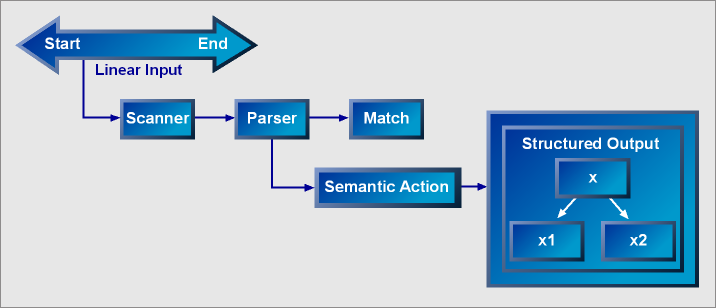
\includegraphics[width=450pt, height=180pt]{./spirit.png}
\caption{Procesos dentro de \spirit}\label{procesoSpirit}
\end{figure}

El usuario es el responsable de definir las ``\texttt{semantic actions}'' para lograr capturar los resultados intermedios, producidos durante la etapa de parsing y no sólo obtener un valor lógico sobre si se pudo o no, consumir toda la cadena de entrada.

Para comenzar a definir una gramática hay que crear una estructura que herede de la clase \texttt{grammar}. Dentro de ella se debe definir a su vez otra estructura templatizada denominada \texttt{definition}. En donde realmente estará la definición de la gramática.

\begin{lstlisting}[language=C++, basicstyle=\scriptsize,numbers=left, numbersep=5pt, numberstyle=\tiny]
struct my_grammar: public grammar <my_grammar>
{
    template <typename ScannerT>
    struct definition
    {
        rule <ScannerT> r;

        definition(my_grammar const& self)
        {
            r = /*... Aqui va la definicion ...*/;
        }
        rule <ScannerT> const& start() const
        {
            return r;
        }
    };
};
\end{lstlisting}

Para definirla, disponemos de un amplio conjunto de herramientas. Primero, los operadores de metalenguaje listados en la tabla \ref{ope_spirit}, los cuales permiten construir nuevas reglas combinando reglas ya definidas, parsers y constantes permitidas en el framework.

\begin{figure}\centering\scriptsize
\begin{tabular}{| c | p{7cm} |}
\hline
\multicolumn{1}{|>{\columncolor[rgb]{0.8, 0.8, 0.8}}l|}{\textbf{Operador}} &
\multicolumn{1}{|>{\columncolor[rgb]{0.8, 0.8, 0.8}}l|}{\textbf{Semántica}} \\ \hline
A $=$                  B  & Definición de A en base a B \\ \hline
A $|$                  B  & Unión, acepta A o B, también llamada ``alternativa''\\ \hline
A $\&$                 B  & Intersección, acepta A y B \\ \hline
A $-$                  B  & Diferencia, acepta A pero no a B  \\ \hline
A $\textasciicircum$   B  & Disyunción exclusiva, acepta A o B, pero no a ambos \\ \hline
A $>>$                 B  & Secuencia, acepta A seguido de B \\ \hline
\multirow{2}{*}{A $\%$ B} & Lista, acepta A separados por ocurrencias de B.\\
                          & Es equivalente a: A $>>$ *(B $>n$ A)\\ \hline
$*$                    A  & Estrella de Kleene, 0 o más veces \\ \hline
$+$                    A  & Positivo, 1 o más veces \\ \hline
$!$                    A  & Opcional, 0 o 1 vez \\ \hline
\end{tabular}
\caption{Operadores de \spirit\ utilizados}\label{ope_spirit}
\end{figure}

Por otra parte, \spirit\ dispone de un gran conjunto de parsers que abarcan la mayoría de los tipos básicos, representación de datos y valores utilizados en el común de los lenguajes (ver tabla \ref{parsers}).

\begin{figure}\centering\scriptsize
\begin{tabular}{| l | l |}
\hline
\multicolumn{1}{|>{\columncolor[rgb]{0.8, 0.8, 0.8}}l|}{\textbf{Parser}} &
\multicolumn{1}{|>{\columncolor[rgb]{0.8, 0.8, 0.8}}l|}{\textbf{Entrada aceptada}} \\ \hline
anychar\_p & Cualquier carácter simple (incluyendo el carácter nulo: '$\setminus0$')\\ \hline
alnum\_p   & Caracteres alfa-numéricos \\ \hline
alpha\_p   & Caracteres alfabéticos \\ \hline
% blank\_p & Un espacio o tabulación \\ \hline
digit\_p   & Dígitos numéricos \\ \hline
lower\_p   & Caracteres en minúscula \\ \hline
upper\_p   & Caracteres en mayúscula \\ \hline
space\_p   & Espacios, tabulaciones, saltos de línea y nuevas líneas \\ \hline
ch\_p      & Carácter especificado como parámetro \\ \hline
str\_p     & Cadena especificada como parámetro \\ \hline
oct\_p     & Dígito en octal \\ \hline
hex\_p     & Dígito en hexadecimal \\ \hline
uint\_p    & Número entero sin signo de 32 bits\\ \hline
int\_p     & Número entero 32 bits\\ \hline
real\_p    & Número flotante 32 bits\\ \hline
eps\_p     & Cadena vacía (épsilon)\\ \hline
end\_p     & Carácter de fin de archivo (EOF)\\ \hline
\end{tabular}
\caption{\label{parsers} Parsers predefinidos de \spirit\ utilizados} 
\end{figure}

Además posee varias directivas que modifican el comportamiento de los parsers, encapsulándose en una expresión definida por el usuario (ver tabla \ref{directivas}).

\begin{figure}\centering\scriptsize
\begin{tabular}{| l | p{7cm} |}
\hline
\multicolumn{1}{|>{\columncolor[rgb]{0.8, 0.8, 0.8}}l|}{\textbf{Directiva}} &
\multicolumn{1}{|>{\columncolor[rgb]{0.8, 0.8, 0.8}}l|}{\textbf{Efecto}} \\ \hline
lexeme\_d    & Deshabilita la omisión de espacios en blanco (space\_p)\\ \hline
as\_lower\_d & Convierte en minúscula lo aceptado por la expresión\\ \hline
\multirow{3}{*}{longest\_d} & Deshabilita el corto circuito, manda al analizador que\\
                            & pruebe todas las alternativas posibles y elija la secuen-\\
                            & cia más larga aceptada \\ \hline
\end{tabular}
\caption{\label{directivas} Directivas de \spirit\ aplicadas}
\end{figure}

Para el manejo de los símbolos válidos dentro de la definición de la gramática, \spirit\ soporta nativamente, el concepto de ``Tablas de símbolos''. Lo que permite registrar de manera dinámica nuevos símbolos, en particular dentro de nuestra herramienta nos ayudó a manejar los conjuntos de nombres válidos para los \texttt{sorts}, los símbolos no terminales permitidos en las ecuaciones, entre otros usos.

Para comenzar a interactuar con el framework, el usuario debe declarar un objeto de la estructura definida y pasarlo como parámetro a una función específica de \spirit.

\begin{lstlisting}[language=C++, basicstyle=\scriptsize, numbers=left, numbersep=5pt, numberstyle=\tiny]
my_grammar g;

if (parse(first, last, g, space_p).full)
{
    cout << "Parsing Succeeded\n";
}
else
{
    cout << "Parsing Failed\n";
}
\end{lstlisting}

\section{Gramática de Atributos con \spirit}

Lo primero que se tuvo que realizar, fue definir los componentes básicos que se iban a necesitar para construir las demás declaraciones.

\begin{description}
\item [Identificadores] son los nombres de sorts, funciones, atributos, símbolos no terminales y reglas, permitidos por \maggen\ y se basan en el común de los estándares. Debido a que el lenguaje del evaluador generado es C++, todas las palabras reservadas de ese lenguaje, son de la misma clase para nuestra herramienta.

\begin{lstlisting}[language=C++, basicstyle=\scriptsize, numbers=left, numbersep=5pt, numberstyle=\tiny]
r_ident = lexeme_d[(alpha_p|'_')>>*(alnum_p|'_')]-r_reserved_word;

r_reserved_word = str_p("compute")|"end"
                | "all"
                | "semantic domain"|"attributes" |"rules"
                | "sort"|"op"|"function"
                | "infix"|"prefix"|"postfix"
                | "syn"|"inh"
                | "left"|"right"|"non-assoc"
                | r_cpp_reserved_words;

r_cpp_reserved_words = r_cpp_basic_types
                     | str_p("and")|"and_eq"|"asm"|"auto"|"bitand"
                     | "bitor"|"break"|"case"|"catch"|"class"|"compl"
                     | "const"|"const_cast"|"continue"|"default"
                     | "delete"|"do"|"double"|"dynamic_cast"|"else"
                     | "enum"|"explicit"|"export"|"extern"|"false"
                     | "for"|"friend"|"goto"|"if"|"inline"|"long"
                     | "mutable"|"namespace"|"new"|"not"|"not_eq"
                     | "operator"|"or"|"or_eq"|"private"|"protected"
                     | "public"|"register"|"reinterpret_cast"|"return"
                     | "short"|"signed"|"sizeof"|"static"|"static_cast"
                     | "struct"|"switch"|"template"|"this"|"throw"|"true"
                     | "try"|"typedef"|"typeid"|"typename"|"union"
                     | "unsigned"|"using"|"virtual"|"void"|"volatile"
                     | "wchar_t"|"while"|"xor"|"xor_eq";

r_cpp_basic_types = str_p("bool")|"char"|"float"|"int"|"string";
\end{lstlisting}

\item [Operadores] Dentro de la especificación de la GA, se permiten como nombre válidos para los operadores, caracteres alfabéticos, numéricos y los operadores básicos de C++. 

\begin{lstlisting}[language=C++, basicstyle=\scriptsize, numbers=left, numbersep=5pt, numberstyle=\tiny]
r_oper = lexeme_d[(alpha_p|'_'|r_id_op)>>*(alnum_p|'_'|r_id_op)];

r_id_op = ch_p('+')|'*'|'/'|'^'|'%'|'&'|'<'|'='|'-'|'>'|'|'|'~'|'.'|','|'?';
\end{lstlisting}

\item [Literales] Son los valores de constantes y tipos básicos aceptados, se adecuan a los estándares de C++. Solamente se tuvo que definir los valores lógicos, los caracteres entre comillas simples y las cadenas de caracteres entre comillas dobles, ya que para los tipos numéricos, existen parsers predefinidos de \spirit\ como ya se dio a conocer.

\begin{lstlisting}[language=C++, basicstyle=\scriptsize, numbers=left, numbersep=5pt, numberstyle=\tiny]
r_boolean = str_p("true")|"false";

r_char = lexeme_d[ch_p('\'')>>(anychar_p)n>ch_p('\'')];

r_string = lexeme_d[ch_p('\"')>>r_string_lit>>ch_p('\"')];

r_string_lit = +((anychar_p-(ch_p('\"')|"\\"|'\'' ))|r_esc_seq);

r_esc_seq = ch_p('\\')>>
            ( oct_p
            | as_lower_d['x']>>hex_p
            | (anychar_p-ch_p('\n'))
            );               
\end{lstlisting}
\end{description}

Para tener una consistencia de identificadores para cada componente de la gramática, utilizamos tablas de símbolos como repositorio, pero también como regla para limitar los posibles valores en posteriores definiciones.

\begin{lstlisting}[language=C++, basicstyle=\scriptsize,numbers=left, numbersep=5pt, numberstyle=\tiny]
symbols <> st_sorts;
symbols <> st_op_prefix;
symbols <> st_op_infix;
symbols <> st_op_postfix;
symbols <> st_functions;
symbols <> st_attributes;
symbols <> st_non_terminal;
\end{lstlisting}

\subsection{\texttt{``semantic domain''} en \spirit}

En esta sección de la especificación se debían aceptar tres tipos de elementos: \texttt{sorts}, \texttt{operators} y \texttt{functions}.

Los \texttt{sorts} serán los tipos que se podrán utilizar para definir los dominios e imágenes de los operadores y funciones.

Según lo explicado en el Diseño, las reglas de cada clase, han sido codificados de la siguiente manera.

\begin{description}
\item [\texttt{sorts}] Exigimos que luego del identificador ``\texttt{sort}'' halla un espacio\footnote{\label{foot:espacio} Ver definición de \texttt{space\_p} \ref{parsers}}. El nombre leído, se usará para crear un nuevo Sort dentro de la GA y también se insertará en la tabla de símbolos de sorts. Se acepta una lista de nombres de sorts para comodidad del usuario.

\begin{lstlisting}[language=C++, basicstyle=\scriptsize, numbers=left, numbersep=5pt, numberstyle=\tiny]
r_decl_sort = lexeme_d[str_p("sort")>>space_p]>>
              (r_ident[&create_sort][st_sorts.add]%',')>>
              ';';
\end{lstlisting}

\item [\texttt{operators}] Para los operadores también se exige el espacio$^{\ref{foot:espacio}}$ luego de la cadena ``\texttt{op}''. Por definición se aceptan tres tipos: infijos, prefijos y posfijos, por lo que se hizo una regla para cada uno, solamente discriminado los dominios, ya que todos poseen una sóla imagen. Notar que los sorts permitidos, son sacados directamente de las tablas de símbolos destinadas para ese propósito.

\begin{lstlisting}[language=C++, basicstyle=\scriptsize, numbers=left, numbersep=5pt, numberstyle=\tiny]
r_decl_oper  = lexeme_d[str_p("op")>>space_p][&inic_func]>>
               (r_oper_infix|r_oper_postfix|r_oper_prefix)>>
               str_p("->")>>
               r_sort_st[&save_image_func]>>
               ';';

r_oper_infix = str_p("infix")[&save_mode_op]>>
               !r_oper_mode>>
               r_oper[&save_name_func][st_op_infix.add]>>
               ':'>>
               r_sort_st[&save_domain_func]>>','>>r_sort_st[&save_domain_func];

r_oper_postfix = str_p("postfix")[&save_mode_op]>>
                 !r_oper_mode>>
                 r_oper[&save_name_func][st_op_postfix.add]>>
                 ':'>>
                 r_sort_st[&save_domain_func];

r_oper_prefix = !(str_p("prefix")[&save_mode_op])>>
                !r_oper_mode>>
                r_oper[&save_name_func][st_op_prefix.add]>>
                ':'>>
                r_sort_st[&save_domain_func];

r_oper_mode = '('>>
               (uint_p[&save_prec_op]|'_')>>
               ','>>
               (r_oper_assoc[&save_assoc_op]|'_')>>
               ')';

r_oper_assoc = str_p("left")|"right"|"non-assoc";
\end{lstlisting}

\item [\texttt{functions}] Para las funciones se permiten como dominio listas de sorts, los cuales serán agregados incrementalmente a la función que se está declarando. La utilización de acciones semánticas facilitan la modularización. La declaración comienza con la cadena ``\texttt{function}'' seguida de una espacio$^{\ref{foot:espacio}}$.

\begin{lstlisting}[language=C++, basicstyle=\scriptsize, numbers=left, numbersep=5pt, numberstyle=\tiny]
r_decl_func = lexeme_d[str_p("function")>>space_p]>>
              r_oper[&inic_func][&save_name_func][st_functions.add]>>
              ':'>>
              !r_dom_func>>
              str_p("->")>>
              r_sort_st[&save_image_func]>>
              ';';

r_dom_func = r_sort_st[&save_domain_func]%',';
\end{lstlisting}
\end{description}

\subsection{\texttt{``attributes''} en \spirit }

Para la codificación de esta sección la funcionalidad buscada era que el usuario mediante una expresión en términos de conjuntos definiera la pertenencia de cada atributo. Por lo que se tuvo que implementar un ``mini-intérprete'' sobre expresiones de conjuntos.

Un detalle a tener en cuenta, en este punto, es que no se encuentra declarado ningún símbolo no terminal'', así que todo símbolo mencionado dentro de la expresión será creado bajo demanda.

La vinculación de los atributos con sus respectivos dueños, se realizará más adelante, debido a que existe la posibilidad de declarar un atributo para todo símbolo, mediante la sentencia \texttt{all}, antes de tener totalmente definido el conjunto de símbolos no terminales de la gramática.

\begin{lstlisting}[language=C++, basicstyle=\scriptsize, numbers=left, numbersep=5pt, numberstyle=\tiny]
r_attributes = lexeme_d[str_p("attributes")>>space_p]>>
               +r_decl_attr[&create_attributes];

r_decl_attr = (r_ident[&add_attribute][st_attributes.add]%',')>>
              ':'>>
              !(r_type_attr[&save_type_attr])>>
              '<'>>r_sort_st[&save_sort_attr]>>'>'>>
              lexeme_d[str_p("of")>>space_p]>>
              (r_conj_symb |
               (str_p("all")n>!('-'>>r_conj_symb))
              )[&save_member_list_attr]>>
              ';';

r_conj_symb = '{'>>(r_ident%',')>>'}';

r_type_attr = str_p("inh")|"syn";
\end{lstlisting}

\subsection{\texttt{``rules''} en \spirit}

En la definición de una gramática las reglas son los pilares, por eso en esta sección se debía brindar la mayor flexibilidad al usuario.

El bloque de reglas comienza con el identificador ``\texttt{rules}'', seguida de un espacio$^{\ref{foot:espacio}}$ y una lista de reglas. Cada una de las mismas son enumeradas desde 1 para mantener una indexación interna. Una vez consumido el bloque se realizan los chequeos que determinan si la GA es MAG o no.

\begin{lstlisting}[language=C++, basicstyle=\scriptsize, numbers=left, numbersep=5pt, numberstyle=\tiny]
r_rules = lexeme_d[str_p("rules")>>space_p]>>
          (+r_decl_rule)>>eps_p[&check_well_defined];
\end{lstlisting}

Una regla individualmente esta representada por un identificador y los caracteres ``\texttt{::=}'' y una lista de símbolos, dejando también la posibilidad de escribir reglas abreviadas mediante el uso del operador ``|'' junto a una nueva lista de símbolos, evitando repetir el lado izquierdo de la regla.

\begin{lstlisting}[language=C++, basicstyle=\scriptsize, numbers=left, numbersep=5pt, numberstyle=\tiny]
r_decl_rule = r_ident[&create_new_non_terminal][&create_rule][st_non_terminal.add]>>
              str_p("::=")>>
              r_right_rule[&save_rule]>>
              *(str_p("|")[&create_abbreviated_rule]>>
              r_right_rule[&save_rule])>>
              ';';
\end{lstlisting}

Dentro de la lista de símbolos se aceptan identificadores de símbolos no terminales y símbolos terminales, definidos mediante una regla específica. Ambos, son creados controlando que no existan repetidos, actualizando la tabla de símbolos solamente de los no terminales.

Se consideran símbolos terminales a cualquier cadena de caracteres encerrada entre comillas simples.

Por definición, una regla puede no contener un bloque de ecuaciones, por lo que es opcional.

\begin{lstlisting}[language=C++, basicstyle=\scriptsize, numbers=left, numbersep=5pt, numberstyle=\tiny]
r_right_rule = +( r_ident[&create_new_non_terminal][st_non_terminal.add]
                | r_terminal[&create_new_terminal]
                )[&save_right_side_rule]>>
               !r_compute_eq;

r_terminal = lexeme_d[ch_p('\'')>>r_string_lit>>ch_p('\'')];
\end{lstlisting}

El mismo estará delimitado por las cadenas \texttt{``compute}'' y \texttt{``end}'', en su interior se aceptará una lista con al menos \textbf{una} ecuación.

Dentro de la definición sólo se podrán utilizar instancias de atributos de los símbolos no terminales que aparecen en la declaración de la regla. Además se debe especificar el índice de ocurrencia, el cual debe cumplir las siguientes condiciones:

\begin{enumerate}
\item Debe ser positivo.
\item El símbolo de la izquierda de la regla tiene el índice 0.
\item Los símbolos no terminales de la parte derecha de la regla, están numerados de izquierda a derecha arrancando en 0 para cada símbolo diferente.
\end{enumerate}

Cada ecuación tiene una instancia de atributo, como ``\texttt{l-value}'', el carácter ``\texttt{=}'' y una expresión como ``\texttt{r-value}''.

\begin{lstlisting}[language=C++, basicstyle=\scriptsize, numbers=left, numbersep=5pt, numberstyle=\tiny]
r_compute_eq = lexeme_d[str_p("compute")>>space_p]>>
               +(r_equation)>>
               str_p("end");

r_equation = r_instance[&create_equation]n>
             '='>>
             r_expression[&save_rvalue]>>
             ';';
\end{lstlisting}

La herramienta acepta cualquier tipo de expresión, ya que se permite que se definan nuevos operadores y funciones según las necesidades de la gramática para la cual se generará el evaluador. Se utilizó la gramática de expresiones ambiguas que figura en la mayoría de los libros de análisis de lenguajes.

\begin{lstlisting}[backgroundcolor=\color{white}]
E := E op E
   | (E)
   | literal
\end{lstlisting}

Donde ``op'' se interpreta como cualquier operador. Esta gramática presentaba el problema de la ``recursión a izquierda'', por lo que se la quitó obteniendo lo siguiente.

\begin{lstlisting}[backgroundcolor=\color{white}]
E := T op1 E
   | T

T := F op2 T
   | F

F := (E)
   | literal
\end{lstlisting}

En nuestra especificación, los ``literales'' pueden ser solamente de tres tipos: funciones, instancias de atributos y los literales propiamente dichos (caracteres, cadenas, valores lógicos, números enteros y flotantes). Los operadores fueron discriminados puntualmente según su sintaxis.

Además, debido a una restricción de \spirit, se tuvo que reescribir toda regla de la forma:

\begin{center}\textbf{\large{$A\ :=\ B\ A\ |\ B\ \ \ \ \Rightarrow\ \ \ \ A\ :=\ B\ (A)*$}}\end{center}

Logrando la siguiente gramática de expresiones, que luego fue codificada en \spirit.

\begin{lstlisting}[backgroundcolor=\color{white}]
E := T (op_infix E)*

T := F (op_postfix)*
   | op_prefix T

F := (E)
   | function
   | literal
   | instance

literal := real
         | int
         | char
         | string
         | bool
\end{lstlisting}

Dentro de las expresiones se tenía que ir resolviendo la precedencia de los operadores declarados por el usuario. Además, la utilización de paréntesis crea distintos niveles de precedencia. Cada vez que se utiliza la producción que genera \texttt{( E )}, la precedencia de los operadores que se utilicen en la expresión \texttt{E}, se resolverán en ese nivel.

\begin{lstlisting}[language=C++, basicstyle=\scriptsize, numbers=left, numbersep=5pt, numberstyle=\tiny]
r_expression = r_expr_prime>>*(r_op_infix_st[&create_operator][&create_func_node]>>
               r_expr_prime[&create_root_infix_node]);

r_expr_prime = r_expr_prime_prime>>
               *(r_op_postfix_st[&create_operator][&create_func_node]
                                [&create_root_postfix_node])
             | r_op_prefix_st[&create_operator][&create_func_node]>>
               r_expr_prime[&create_root_prefix_node];

r_expr_prime_prime = ch_p('(')[&increment_level]>>
                        r_expression>>
                     ch_p(')')[&decrement_level]
                   | r_function[&create_root_function_node]
                   | r_literal[&create_literal_node]
                   | r_instance[&create_instance_node];
\end{lstlisting}

Las definiciones de los tres tipos de literales son coherentes con el estilo de codificación que se usó hasta el momento.

Las funciones aceptan expresiones como parámetros, así que, la asociatividad y precedencia de esas expresiones se resuelve entre los paréntesis explícitos que se exigen en la invocación a una función.

Al completar esta regla se creará una \texttt{Expr\_function} dentro de la gramática.

\begin{lstlisting}[language=C++, basicstyle=\scriptsize, numbers=left, numbersep=5pt, numberstyle=\tiny]
r_function = r_function_st[&create_function][&create_func_node]>>
             ch_p('(')[&push_mark][&increment_level]>>
             !(r_expression%',')>>
             ch_p(')')[&decrement_level];
\end{lstlisting}

Aprovechando las funcionalidades de \spirit, se resolvió una ambigüedad al momento de parser un número entero y un flotante, exigiendo que se quede con la cadena más larga que pudiese coincidir en la gramática. Para ello se codificó lo siguiente:

\begin{center}\textbf{\large{\texttt{longest\_d\ [\ real\_p\ |\ int\_p\ ]}}}\end{center}

Utilizando la directiva \texttt{longest\_d} sobre la unión de ambos parsers predefinidos para dichos valores numéricos.

Para los demás literales se usaron las reglas definidas en un comienzo de la gramática.

Luego de parsear cada uno de los literales se crean los respectivos objetos dentro del ambiente de tipo \texttt{Expr\_literal}.

\begin{lstlisting}[language=C++, basicstyle=\scriptsize, numbers=left, numbersep=5pt, numberstyle=\tiny]
r_literal = longest_d[real_p|int_p][&create_lit_number]
          | r_char[&create_lit_ch]
          | r_string[&create_lit_str]
          | r_boolean[&create_bool];
\end{lstlisting}

Una instancia debe ser un bloque que contenga una ocurrencia de un símbolo y un atributo del mismo. Por lo que no se aceptan espacios intermedios. Se utilizó la directiva \texttt{lexeme\_d}.

Con los datos obtenidos se crea un objeto de tipo \texttt{Expr\_instance}.

\begin{lstlisting}[language=C++, basicstyle=\scriptsize, numbers=left, numbersep=5pt, numberstyle=\tiny]
r_instance = lexeme_d[
               r_non_term_st[&create_instance]>>
               '['>>int_p[&save_index_ins]>>']'>>
               '.'>>r_attribute_st[&save_attr_ins]
             ];
\end{lstlisting}

En este punto se encuentran definidas todas las reglas necesarias para declarar la regla que define a una \textbf{Gramática de Atributos}. Es decir, un dominio semántico, un bloque de atributos y un bloque de reglas. El parser \texttt{end\_p} se necesita para que consuma los espacios restantes hasta el fin del archivo de entrada.

\begin{lstlisting}[language=C++, basicstyle=\scriptsize, numbers=left, numbersep=5pt, numberstyle=\tiny]
r_att_grammar = r_semantic_domain >>
                r_attributes >>
                r_rules >>
                end_p;
\end{lstlisting}

Por cuestiones de diseño de \spirit, no se podían aplicar acciones semánticas a las tablas de símbolos, por lo que se crearon reglas auxiliares para mediar de puente.

A excepción de la regla que se utilizó para definir los identificadores válidos para un \texttt{sort}, a la que se le agregaron los tipos básicos soportados por \maggen.

\begin{lstlisting}[language=C++, basicstyle=\scriptsize, numbers=left, numbersep=5pt, numberstyle=\tiny]
r_sort_st       = st_sorts|r_cpp_basic_types;
r_op_prefix_st  = st_op_prefix;
r_op_infix_st   = st_op_infix;
r_op_postfix_st = st_op_postfix;
r_function_st   = st_functions;
r_attribute_st  = st_attributes;
r_non_term_st   = st_non_terminal;
\end{lstlisting}

\subsection{Comentarios}

Para incorporar los dos estilos de comentarios de C++, se definió una gramática que los aceptara y se utilizó como el parser para todos las cadenas que se omiten dentro del archivo de entrada.

\begin{lstlisting}[language=C++, basicstyle=\scriptsize, numbers=left, numbersep=5pt, numberstyle=\tiny]
struct skip_parser: public grammar <skip_parser>
{
  template <typename ScannerT>
  struct definition
  {
    definition(skip_parser const &self)
    {
      skip = space_p
           | "//" >> *(anychar_p - '\n')
           | "/*" >> *(anychar_p - "*/") >> "*/"
           ;
    }
    rule <ScannerT> skip;

    rule <ScannerT> const &start() const
    {
      return skip;
    }
  };
};
\end{lstlisting}

La invocación a la funcionalidad de \spirit\ se realiza con una instancia de \texttt{attritute\_grammar}, como gramática objetivo, y otra de \texttt{skip\_parser}, como parser de omisión.

\begin{lstlisting}[language=C++, basicstyle=\scriptsize, numbers=left, numbersep=5pt, numberstyle=\tiny]
attritute_grammar  attr_grammar_decl;
skip_parser        skip_p;

parse_info<iterator_t> info(parse<iterator_t>(begin, end, attr_grammar_decl, skip_p));
\end{lstlisting}

\subsection{Manejo de errores}

Para informar los errores durante el análisis sintáctico, teníamos que utilizar los mecanismos que \spirit\ nos brindaba. Lamentablemente este es un punto débil del framework.

Lo que se implementó, fue mostrar la línea y columna desde donde no se pudo consumir del archivo de entrada.

Primero, para aceptar archivos como entrada de la herramienta, se tiene que hacer que \spirit\ no utilice un iterador estándar, sino que un \texttt{file\_iterator} instanciado con caracteres. Luego definir un \texttt{position\_iterator} sobre el recién mencionado.

De esta forma, el parser que se invocará para que analice la entrada de \maggen, lo hará moviéndose mediante este iterador y ante cualquier error, se podrá obtener la última posición parseada correctamente.

\begin{lstlisting}[language=C++, basicstyle=\scriptsize, numbers=left, numbersep=5pt, numberstyle=\tiny]
typedef char                           char_t;
typedef file_iterator <char_t>         iterator_f;
typedef position_iterator <iterator_f> iterator_t;
\end{lstlisting}

\subsection{Observaciones}

Toda la implementación del analizador sintáctico de \maggen\ está dentro del directorio ``Parser'', en el que se encuentran los siguientes archivos:

\begin{description}
\item [Parser.cpp] En el que se encuentran todas las estructuras comentadas en la sección anterior.

\item [Semantics\_actions.cpp] Aquí se implementaron todas las acciones semánticas que se utilizan durante el análisis sintáctico para ir creando los objetos que internamente representan y componen a una Gramática de Atributos.

\item [Semantics\_checks.cpp] Simultáneamente con el parser, se realizan chequeos de propiedades sobre las reglas que se consumieron completamente. Dichos algoritmos se encuentran implementados en este archivo. Ahora se mencionarán detalles sobre los mismos.
\end{description}

\section{Chequeos semánticos durante el parsing}

Dentro de este módulo se mantienen las variables que almacenan el nivel de precedencia corriente durante el parsing. El mismo es inicializado en 0 (cero), se incrementa en 1 (uno) cada vez que se detecta un paréntesis que abre y se decrementa al encontrar uno que cierra.

Además, para enumerar los símbolos que van apareciendo dentro de las reglas, se mantiene un índice se aparición sintáctico. Comienza en 0 (cero) y se incrementa cada vez que se consume un símbolo dentro de la declaración de la regla.

Ambos valores numéricos son reseteados cada vez que se comienza a analizar una nueva regla.

\subsection{Solución a problemas de precedencia de operadores}

Mientras se parsea una expresión se busca mantener la propiedad de que los \textbf{operadores de mayor precedencia se apliquen antes que otros con menor}. Por lo que cada vez que se detecta un nuevo operador, se debe evaluar si se tiene que realizar modificaciones al árbol armado hasta el momento, aparte de la inserción del operador y sus argumentos.

Cuando se presenta un problema de precedencia, se realizan rotaciones que se aplican recursivamente en todo el árbol. 

Los cambios mantienen invariante la propiedad de que no se afecta al orden sintáctico de la expresión, es decir, el aplanamiento del árbol de izquierda a derecha (in-order) es el mismo antes y después de las permutaciones.

\begin{figure}\centering
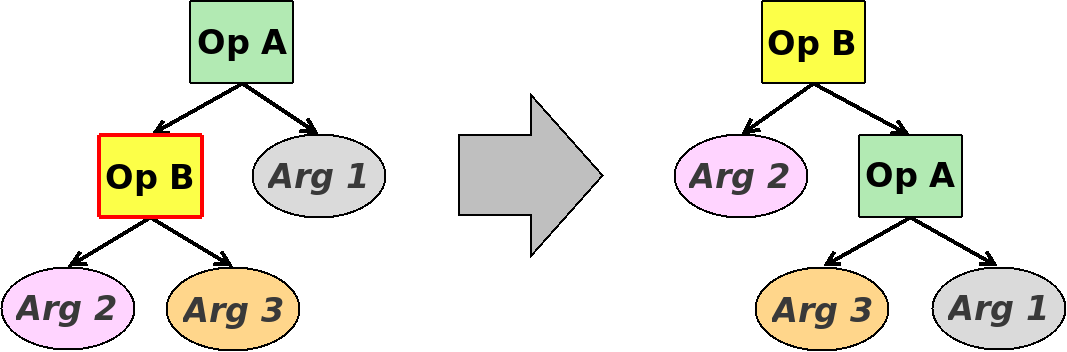
\includegraphics[width=250pt, height=82pt]{./rotacion1.png}
\caption{\label{rotacion1} Caso de rotación cuando la operación de la izquierda tiene menor precedencia.}
\end{figure}

\begin{figure}\centering
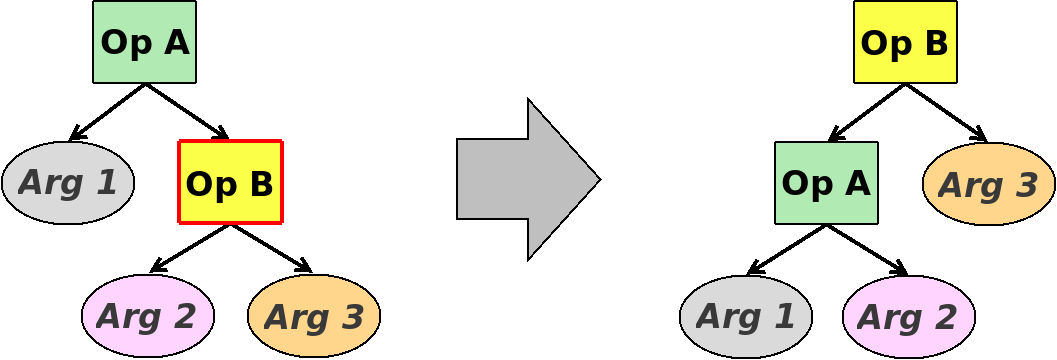
\includegraphics[width=250pt, height=85pt]{./rotacion2.png}
\caption{\label{rotacion2} Caso de rotación cuando la operación de la derecha tiene menor precedencia.}
\end{figure}

\begin{figure}\centering
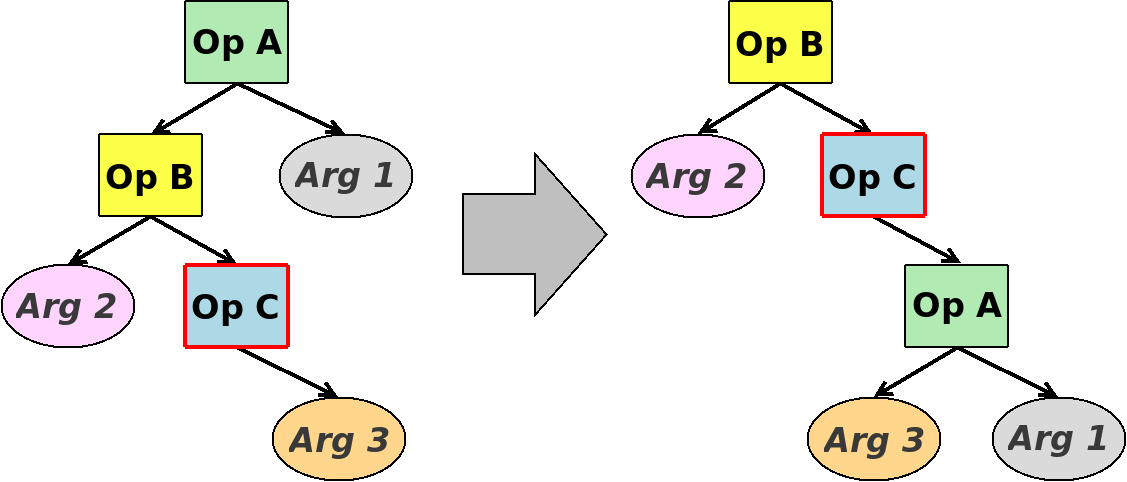
\includegraphics[width=250pt, height=107pt]{./rotacion3.png}
\caption{\label{rotacion3} Caso de rotación cuando se detectó un conflicto sin resolver.}
\end{figure}

Existen dos grandes casos a considerar:
\begin{itemize}
\item Si se inserta una operación infija, como hijo de otra operación, pero con menor precedencia que su padre, entonces se modificará el árbol, dejando como nueva raíz la operación infija recién insertada. 

Existen dos variantes, las cuales son presentadas en los diagramas \ref{rotacion1} y \ref{rotacion2}.

\item En cambio, cuando se inserta cualquier operación como hija de una operación prefija (raíz) y la insertada tiene mejor precedencia que la raíz, no se resuelve instantáneamente el error, dado que se alteraría el orden sintáctico de la expresión. Para ello se prende una bandera, a la cual se le asigna el valor de precedencia que tiene la operación recién insertada. Entonces cuando en el siguiente paso se agregue una nueva raíz, si tiene mayor precedencia que su ``nieto'' en el árbol, se realiza la siguiente rotación mostrada en el diagrama \ref{rotacion3}.
\end{itemize}

\subsection{Asociatividad de operadores dentro de expresiones}

El chequeo de la asociatividad y las eventuales modificaciones en el árbol de expresión, a diferencia del tratamiento que se le da a los problemas de precedencia, no se realiza a medida que se obtiene el árbol, sino que se lo aplica solamente una vez, cuando ya se terminó de parsear la expresión.

Esto se implementó así, ya que en ese punto, todos los elementos del árbol se encuentran posicionados respetando todas las precedencias, quedando potencialmente inconsistente la asociación de dos o más operadores infijos iguales, dentro del mismo nivel sintáctico, y con asociatividad a \textbf{derecha}, ya que por defecto todos los operadores son asociados a izquierda, debido al parser descendente recursivo que aplica \spirit.

Además, cuando se detectan dos operadores no asociativos se genera un error por mal uso de ese operador dentro de la expresión. Tal como se analizó en la sección XXX.

\subsection{Alcanzabilidad de símbolos y reglas}

En la especificación pueden existir de símbolos y reglas declaradas que no pueden ser alcanzados desde el símbolo inicial de la gramática. Los mismos no son útiles en la gramática ya que nunca producirán cadenas del lenguaje. Los mismos no son considerados errores pero son informados mediante alertas (\texttt{warnings}).

Este chequeo se implementó con una versión del algoritmo de Warshall\footnote{En honor a Stephen Warshall (1935 - 2006)}, que calcula la ``Clausura Transitiva'' de un grafo.

Para aplicarlo, primero se construye una matriz de valores lógicos reflejando todas las reglas declaradas. Luego de computar la clausura, se recorre la fila del símbolo inicial, que pertenece a la \textbf{única} regla inicial de la gramática por ser \textbf{extendida}. Todo símbolo que se encuentra con valor falso es inalcanzable.

\subsection{Consistencia de bloque de atributos y bloque de reglas}

Este chequeo consiste en verificar que no existan símbolos declarados en el bloque de atributos, que no hallan sido involucrados en ninguna regla. Esto puede suceder se crearon los símbolos de la expresión de conjuntos que define la pertenencia de un atributo.

La heurística utilizada, consiste en recorrer el \texttt{map} de símbolos no terminales y verificando que existe al menos una regla que lo tenga como parte izquierda.

\subsection{Gramática bien definida}

Este control es uno de los más importantes, ya que si la gramática por más que haya sido parseada correctamente, si no cumple con las condiciones de una MAG, nuestra herramienta la descarta y no le generará su correspondiente evaluador.

Como ya me sencionó en el capítulo XXX, varias son las condiciones que se deben chequear.

La heurística aplicada fue recorrer el \texttt{map} de reglas, donde para cada una verificábamos que estuviesen definidas dentro de su \texttt{map} de ecuaciones, una para cada uno de sus atributos sintetizados. Y a su vez, una ecuación para cada atributo heredado de sus símbolos de la parte derecha.

Además, también se controlara que no existieran ecuaciones incorrectas, es decir:
\begin{itemize}
\item Ecuaciones para atributos heredados del símbolo de la izquierda.
\item Ecuaciones para atributos sintetizados de símbolos de la parte derecha.
\end{itemize}

Cada vez que se detectaba un error, se lo informa mediante alguno de los siguientes mensajes según corresponda.

\texttt{\begin{itemize}
\item ``ERROR: ``E[1].syn1'' type synthetized, haven't an equation that defines it.''
\item ``ERROR: ``S[0].inh1'' type inherited, is defined outside his scope.''
\item ``ERROR: ``E[1].inh2'' type inherited, haven't an equation that defines it.''
\item ``ERROR: ``S[0].syn2'' type synthetized, is defined outside his scope.''
\end{itemize}}


\section{Obtención de planes de evaluación}

Como ya se explicó en el diseño, el propósito final de \maggen\ es obtener todos los planes posibles de la gramática de entrada.

Los planes están representamos como una secuencia de identificadores de ecuaciones. Utilizando la clase \texttt{vector} de la STL y manteniendo la unicidad en la enumeración de las ecuaciones.

Como en general, se iban a generar en muchos casos los mismos planes, se desidió mantener un \texttt{vector} con todos los planes diferentes, así solo generaríamos la mínima cantidad de planes únicos.

Como en el algoritmo que se presenta en el artículo de Wuu Yang(ver bibliografía XXX), a cada plan se lo asocia con un \texttt{key}, primero implementamos esa clave como una estructura con los siguientes datos:
\begin{itemize}
\item La regla a la cual pertenece el plan
\item Una secuencia para computar sus atributos
\end{itemize}

Esa secuencia se representó de igual manera que un plan, ya que computar un atributo es equivalente a saber el identificador de la ecuación que lo tiene como \texttt{l-value}.

El conjunto de estas secuencias, son los planes proyectados, es decir, las exigencias que se le imponen a una regla desde un contexto superior que la invoca a que se compute. Para el símbolo inicial, esta secuancia es obtenida como el órden topológico de su grafo DCG, ya que este contiene todas las dependencias entre los atributos de la regla, el cual si o si, será un órden de computación consistente para sus ecuaciones.

Al igual que con los planes de evaluación, los planes proyectados también sufrían de muchas repeticiones, por lo cual se usaron índices indirectos a un repositorio de los mismos almacenados en un \texttt{vector}.

Cada plan proyectado estaba bajo una clave particular, la cual según el algoritmo debía contener:
\begin{itemize}
\item La regla a la cual pertenece el plan proyectado
\item Una secuencia para computar sus atributos
\item El símbolo con el cual se proyento el plan de evaluación
\end{itemize}

Los dos primeros valores, corresponden a un \texttt{key} de un plan de evaluación, asi que se usó directamente esa estructura.

\subsection{Construcción de grafos}

Para la representación de los grafos uitlizamos la \boost\ \textit{\textbf{Graph Library}} (\textbf{BGL}). Ya que la misma presentaba muchas funcionalidades y ya se encontraba como una dependencia externa de la herramienta.

Como en la mayoria de los componentes de esta biblioteca, los mismos eran plantillas que necesitaban ser instanciados.

Las dependencias dentro de las reglas se dan entre las instancias de atributos de las ecuaciones y además los literales.

En la \textbf{BGL} los valores que se quieren asociar a los nodos, se vinculan mediante \textit{propiedades} inherentes a cada uno.

\begin{lstlisting}[language=C++, basicstyle=\scriptsize, numbers=left, numbersep=5pt, numberstyle=\tiny]
struct vertex_data_t
{
    typedef vertex_property_tag kind;
};
typedef property <vertex_data_t, const genevalmag::Expr_leaf*> property_vertex_dp;
typedef adjacency_list <hash_setS, vecS, directedS, property_vertex_dp> Graph;
typedef Graph::vertex_descriptor Vertex;
\end{lstlisting}

Se mantienen dentro de la herramienta un \texttt{map} para cada uno de los tipos de grafos necesarios y además para los subgrafos ADP cíclicos que eventualmente se detecten y para optimizar la construcción de los otros, los grafos que contienen todas las instancias de cada regla sin aristas entre si.

\begin{lstlisting}[language=C++, basicstyle=\scriptsize, numbers=left, numbersep=5pt, numberstyle=\tiny]
map <string, Graph>                 attr_vertex_graphs;
map <unsigned short, Graph>         p_Dp_graphs;
map <string, Graph>                 p_Down_graphs;
map <unsigned short, Graph>         p_Dcg_graphs;
map <vector<unsigned short>, Graph> p_Adp_graphs;
map <vector<unsigned short>, Graph> p_Adp_subgraphs_cyclics;
\end{lstlisting}

El chequeo de ciclicidad sobre los grafos ADP, se implementó utilizando el algoritmo de búsqueda en profundidad (Depth-first search) de \boost\ combinado con la creación de un ``visitador'' especilizado que a medida recorre el grafo, va guardado los nodos y aristas visitadas mientras no se halla detectado un ciclo. Ese subgrafo es lo que se guarda y se muestra al usuario.

La detección de ciclos se realiza cuando el algoritmo invoca a la función \texttt{back\_edge}, en donde nosotros prendemos una bandera.

Tanto el grafo como la variable lógica, usada como bandera, son pasadas en el constructor y utilizadas internamente mediante referencias.

\begin{lstlisting}[language=C++, basicstyle=\scriptsize, numbers=left, numbersep=5pt, numberstyle=\tiny]
struct cycle_detector: public dfs_visitor<>
{
  public:
    cycle_detector(bool& has_cycle, Graph &graph):
      _has_cycle(has_cycle),
      _graph_cycle(graph)
    {}

    template <class Edge, class G>
    void examine_edge(Edge u, const G &g)
    {
      if(!_has_cycle)
      {
        ...
      }
    }

    template <class Edge, class G>
    void back_edge(Edge u, const G& g)
    {
      _has_cycle = true;
    }

  protected:
    bool   &_has_cycle;
    Graph  &_graph_cycle;
};
\end{lstlisting}

Para cada regla, se tienen que considerar todos los posibles contextos inferios posibles de acuerdo a las reglas que tengan los símbolos no terminales de su parte derecha. Se implementó un método que recursivamente genera un contexto diferente y guarda la regla cuando ya no quedan más variantes.

Al igual que con los planes, los contextos de las reglas se repiten mucho, así que se utilizaron índices indirectos sobre un \texttt{vector} que almacena unicamente los contextos diferentes.

\begin{lstlisting}[language=C++, basicstyle=\scriptsize, numbers=left, numbersep=5pt, numberstyle=\tiny]
vector < Order_rule >    contexts_uniques;
vector < Order_eval_eq > plans_uniques;
vector < Order_eval_eq > plans_project_uniques;
\end{lstlisting}

Antes de insertar un elemento en cualquiera de estos repositorios se verifica que no exista. En caso de que ya se encuentre, se devuelve el índice correspondiente dentro del vector, sino se insertará al final y se devolverá el índice del último elemento.

Una vez que se generaron todos los tipos de grafos, los mismos son guardados en distintos directorios en formato \textbf{dot}\cite{dot}. Para ello utilizamos la función \texttt{write\_graphviz} perteneciente a al módulo Graphviz de \boost.

La generación de grafos es incremental, partiendo de la computación de los grafos DP, siguiendo los Down, DCG y por último los grafos ADP. Ante cualquier fallo, la generación se considerará incompleta.

\begin{lstlisting}[language=C++, basicstyle=\scriptsize, numbers=left, numbersep=5pt, numberstyle=\tiny]
bool generate_graphs()
{
  if(build_graphs.compute_dependency_graphs())
  {
    if(build_graphs.compute_down_graph())
    {
      if(build_graphs.compute_dcg())
      {
        if(build_graphs.compute_adp_graph())
        {
          cout << "* Generate graphs ---------- [  OK  ]" << endl;
          return true;
        }
      }
    }
  }
  cout << "* Generate graphs ---------- [ FAIL ]\n" << endl;
  return false;
}
\end{lstlisting}

Una vez que se concluyó la generación de grafos, se construyen los planes, se prosigue con el chequeo de ciclicidad de los grafos ADP. Si se supera con éxito, se generarán los planes, sino se abortará el proceso.

\begin{lstlisting}[language=C++, basicstyle=\scriptsize, numbers=left, numbersep=5pt, numberstyle=\tiny]
unsigned short build_plans()
{
  if(generate_graphs())
  {
    if (build_graphs.check_cyclic_adp_dependencies())
    {
      cout << "* Build plans -------------- [ ABORT ]\n" << endl;
      return 1;
    }
    else if(generate_plans())
    {
      cout << "* Build plans -------------- [  OK  ]" << endl;
      return 0;
    }
    cout << "* Build plans -------------- [ FAIL ]\n" << endl;
  }
  return 2;
}
\end{lstlisting}

El proceso de construir un plan es complejo, la heurística seguida respeta el algoritmo para computar planes presentado por Wuu Yang (ver XXX).

Por lo que se implementaron las funciones y elementos involucrados con lo siguiente:

\begin{itemize}
\item Lista de trabajos: \textbf{WL} \flecha \texttt{vector <Item\_work>\ work\_list;}
\item Trabajos realizados: {\LARGE\textbf{$\Delta$}} \flecha \texttt{vector <Item\_work>\ defined\_item\_work;}
\item Función que computar un orden de evaluación de ecuaciones: \textbf{ComputeOrder} \flecha \texttt{compute\_order}
\item Función que filtra del orden total sólo lo para un símbolo: \textbf{Project} \flecha \texttt{purge\_plan\_with}
\item Planes de evaluación: {\LARGE\textbf{$\Theta$}} \flecha \texttt{map <Key\_plan, unsigned short>\ eval\_plans;}
\item Planes de evaluación proyectados: {\LARGE\textbf{$\gamma$}} \flecha \texttt{map <Key\_plan\_project, unsigned short>\ plans\_project;}
\end{itemize}

\normalsize
